%\chapter{Visualização volumétrica}
\chapter{Volume Rendering}
\label{cap:vis_vol}

For volume rendering models, has a InVesalius employs a technique known as raycasting. In summary, Raycasting is it a technique to simulate the trace a beam of light toward the object for each screen pixel. The pixel color is based on the color and transparence of each voxel intercepted by the light beam.


%No InVesalius, existem diversos padrões pré-definidos (\textit{presets}) para visualizar
%determinados tipos de tecidos ou diferentes tipos de exames (tomografia com contraste, por
%exemplo).

In InVesalius, there are several pre-defined patterns (presets) to display specific tissue types or different types of tests (tomographic contrast, for example).

%Para acessar esse recurso, basta clicar no atalho ilustrado pela figura
%\ref{fig:volume_raycasting_origina}, localizado no canto inferior direito da tela (ao lado da
%janela de exibição de superfícies) e selecionar um dos padrões disponíveis.

To access this feature, simply click the shortcut shown in figure~\ref{fig:volume_raycasting_origina} in the lower right corner of the screen (next to the display window surfaces) and select one of the available standards.

%Para desativar a visualização volumétrica, clique novamente no atalho indicado pela figura
%\ref{fig:volume_raycasting_origina} e escolha a opção \textbf{Desabilitado}.

To turn off the volume rendering, click again on the path indicated by the figure~\ref{fig:volume_raycasting_origina} and select the Disabled option.

\begin{figure}[!htb]
\centering

\includegraphics[scale=0.4]{volume_raycasting_origina}
\caption{Shortcut to volume visualization}
\label{fig:volume_raycasting_origina}
\end{figure}

%\section{Padrões de visualização}
\section{Viewing Standards}

%São diversos os padrões de visualização pré-definidos. Alguns exemplos são ilustrados nas
%figuras seguintes.
There are several predefined viewing patterns. Some examples are illustrated in the following figures. 

\begin{figure}[!htb]
\centering
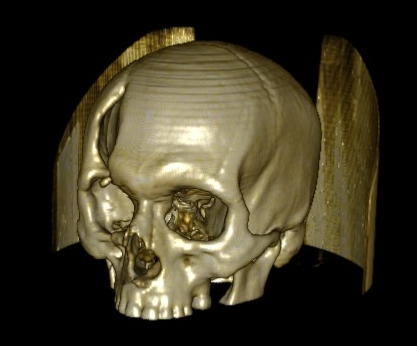
\includegraphics[scale=0.68]{brilhante_I}
\caption{Bright}
\label{fig:brilhante_I}
\end{figure}

\begin{figure}[!htb]
\centering 
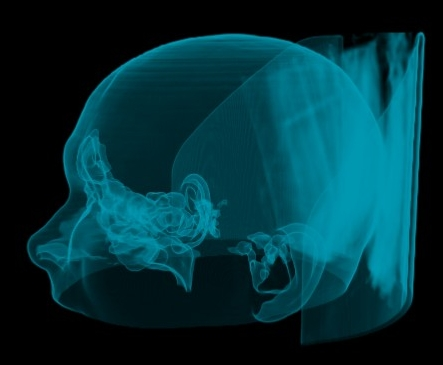
\includegraphics[scale=0.65]{vias_aereas_II}
\caption{Airway II}
\label{fig:vias_aereas_II} 
\end{figure}

\begin{figure}[!htb]
\centering
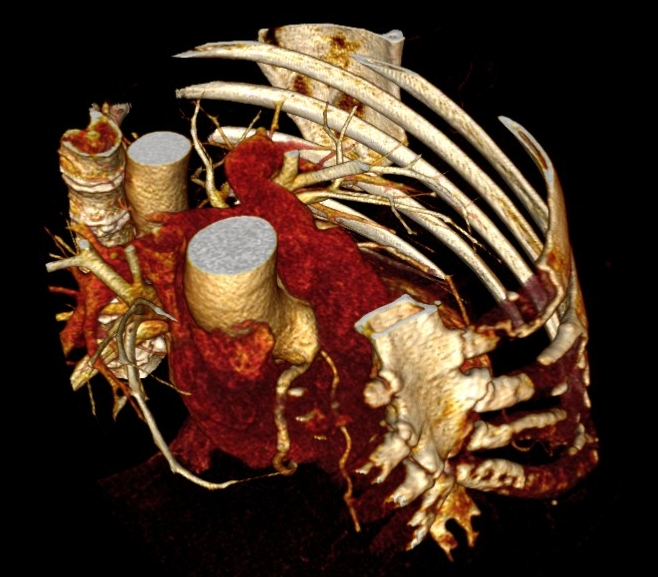
\includegraphics[scale=0.42]{contraste_medio}
\caption{Contrast Medium}
\label{fig:contraste_medio}
\end{figure}

\begin{figure}[!htb]
\centering
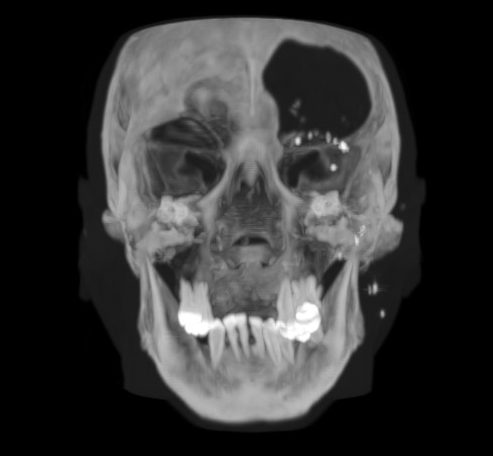
\includegraphics[scale=0.55]{MIP}
\caption{MIP}
\label{fig:MIP}
\end{figure}


\newpage


%\section{Personalização de padrão}
\section{Standard Customization}

%Alguns padrões podem ser personalizados (ou customizados). Veja a figura
%\ref{fig:customize_1}, que exibe um padrão e alguns controles gráficos de ajuste.
%Com eles, é possível alterar a cor de uma dada estrutura e sua opacidade, determinando
%como e se ela será exibida.
Some patterns can be personalized (and customized). See figure~\ref{fig:customize_1}, which is exhibiting a pattern and some graphical controls adjustment. With these features, It is possible to change the color of a given structure and its opacity, determining if and how it will be displayed.

\begin{figure}[!htb]
\centering
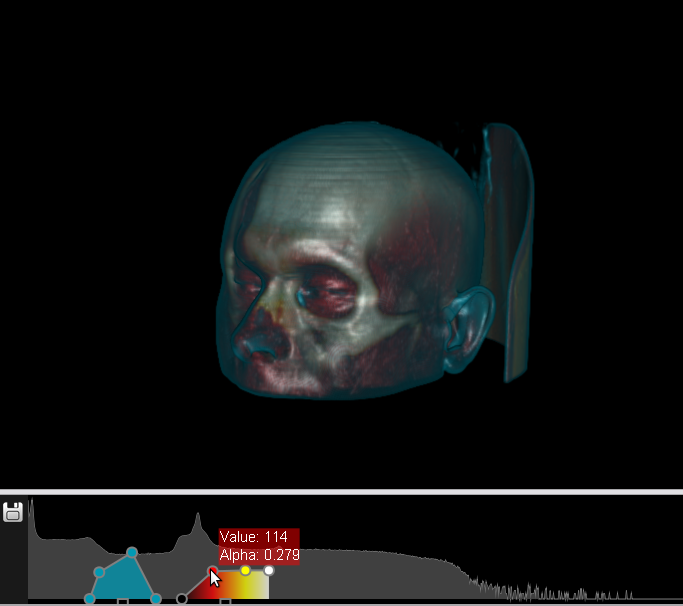
\includegraphics[scale=0.6]{customize_1}
\caption{Settings for the display pattern Soft Skin + II}
\label{fig:customize_1}
\end{figure}


\newpage


%Caso se deseje ocultar uma estrutura, é necessário utilizar o controle gráfico de ajuste mantendo
%baixa a opacidade da região correspondente. No exemplo da figura \ref{fig:customize_1},
%suponha que se pretende esconder a parte muscular, que aparece em vermelho. Para isso, basta
%posicionar o ponteiro do mouse sobre o ponto em vermelho e, com o botão esquerdo pressionado,
%\textbf{arrastar} o ponto para baixo, a fim de diminuir a opacidade (o que equivale a aumentar
%a transparência). A figura \ref{fig:customize_2} ilustra o resultado.

To hide a structure, you must use the control setting chart keeping low the opacity of the corresponding region. In the example in figure~\ref{fig:customize_1} for example, suppose you want to hide the muscular part, which appears in red. To do this, one can simply position the pointer over the point in red and using the left mouse button, drag the point down in order to reduce the opacity (which is equivalent to increasing transparency). Figure~\ref{fig:customize_2} illustrates the result.

%Nota: O valor \textit{Alpha} indica a opacidade da cor, e o valor \textit{Value}, a
%intensidade da cor no pixel.

Note: The Alpha value indicates the opacity of the color and the value Value, the color intensity of the pixel.

\begin{figure}[!htb]
\centering
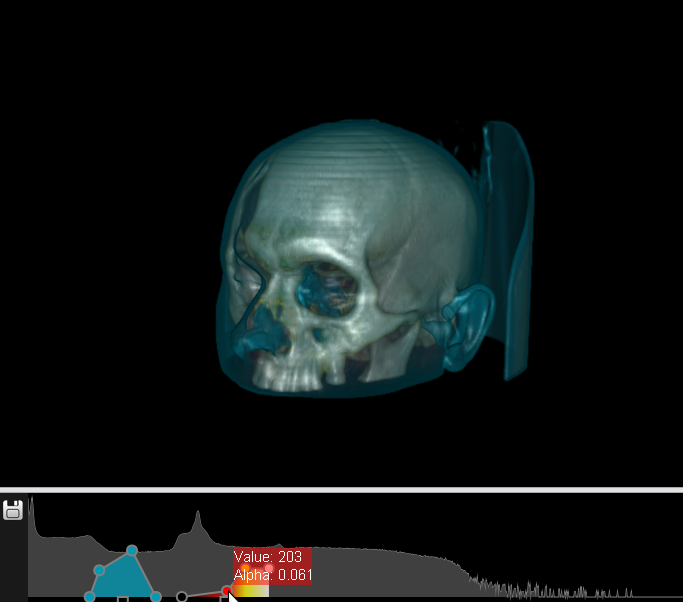
\includegraphics[scale=0.6]{customize_2}
\caption{Display Standard Soft Skin + II changed}
\label{fig:customize_2}
\end{figure}


\newpage


%É possível remover ou adicionar pontos no controle gráfico de ajuste. Para a remoção, basta clicar
%com o botão \textbf{direito} do mouse sobre o ponto. Para adicionar um novo ponto, clique com
%o botão \textbf{esquerdo} sobre a linha do gráfico. Pode-se também salvar o padrão resultante,
%clicando no atalho que a figura \ref{fig:save_preset} ilustra.

It can remove or add points on the graph control setting. For removing, simply click with the right mouse button on the point. For adding a new point, click the left button on the line
graph. One can also save the resulting pattern by clicking the shortcut.  Figure~\ref{fig:save_preset} illustrates.

\begin{figure}[!htb]
\centering

\includegraphics[scale=0.6]{save_preset}
\caption{Shortcut to save standard}
\label{fig:save_preset}
\end{figure}
 
%Ao salvar o padrão, o InVesalius exibe uma janela como a da figura \ref{fig:save_window_preset}.
%Digite um nome para o padrão personalizado e clique em \textbf{OK}. O padrão salvo estará
%disponível com os demais na próxima vez em que o software for aberto.

To save the pattern, InVesalius displays a window like the one in figure~\ref{fig:save_window_preset}.
Enter a name for the custom pattern and click OK. The saved pattern will be available with the other the next time the software is opened.

\begin{figure}[!htb]
\centering
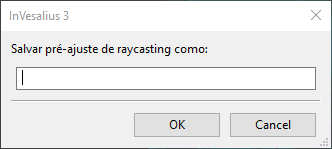
\includegraphics[scale=0.7]{save_window_preset_pt.png}
\caption{The image shows the Window to name and save a pattern.}
\label{fig:save_window_preset}
\end{figure}

%\section{Personalização de padrão com Brilho e Contraste}
\section{Standard Customization with Brightness and Contrast}

%É possível personalizar um padrão sem utilizar o controle gráfico de ajuste, apresentado na seção
%anterior. Isso é feito por meio do controle de brilho e \textbf{Contraste} presente na barra de
%ferramentas. Para ativar o controle, clique no atalho ilustrado pela figura
%\ref{fig:tool_contrast_original_vol}.

You can customize a pattern without using the graphical control setting, which is presented in the previous section. This is done through the brightness control and contrast which is present in the toolbar. To activate the control, click the shortcut shown in figure~\ref{fig:tool_contrast_original_vol}.

\begin{figure}[!htb]
\centering

\includegraphics[scale=0.6]{tool_contrast_original}
\caption{Shortcut to Brightness and Contrast}
\label{fig:tool_contrast_original_vol}
\end{figure}

%Com o controle ativado, arrastando o mouse com o botão esquerdo pressionado
%sobre a janela do volume, é possível alterar os valores de \textit{window width} e
%\textit{window level}. O procedimento é o mesmo aplicado para as fatias 2D, visto
%na seção \ref{sec:ww_wl}. Arrastando o mouse na direção horizontal, altera-se o valor de
%\textit{window level}. Para a esquerda, diminui-se seu valor e, para a direita,
%aumenta-se seu valor. Arrastando o mouse na direção vertical, altera-se o valor de
%\textit{window width}. Para baixo, diminui-se seu valor e, para cima, aumenta-se seu
%valor.

Enable the control by dragging the mouse, with the left button pressed on the volume window, this can change the values of the window width and window level. The procedure is the same as the slices applied to 2D, which can be seen in section~\ref{sec:ww_wl}. Dragging the mouse in the horizontal direction changes  the window level value. To the left, it decreases its window value, and for the right, it increases its window value. Dragging the mouse in the vertical direction changes the value of window width. If dragged down, the value is diminished and, dragging upwards increases its value.

%Com a manipulação desses valores, conseguem-se diferentes resultados de
%visualização. Por exemplo, para adicionar tecido à visualização, \textbf{arraste} o
%mouse diagonalmente, do canto inferior direito para o canto superior esquerdo da janela
%de visualização. Para remover tecido da visualização, faça o contrário, ou seja,
%\textbf{arraste} o mouse diagonalmente, do canto superior esquerdo para o canto inferior
%direito. Veja a figura \ref{fig:raycasting_add}.

Manipulating these values can be useful for different viewing results. For example, to add tissue to the display, drag the mouse diagonally from the lower right to the upper left corner of the preview window. To remove tissue visualization, do the opposite, (i.e drag the mouse diagonally from top left to bottom Right.). See figure~\ref{fig:raycasting_add}.

\begin{figure}[!htb]
  \centering
  \subfloat[Bone]{\label{fig:raycasting_add_1}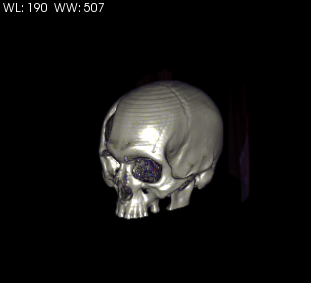
\includegraphics[width=0.33\textwidth]{raycasting_add_1}}                
  \hfill
  \subfloat[Muscle]{\label{fig:raycasting_add_2}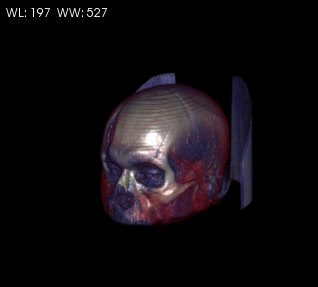
\includegraphics[width=0.333\textwidth]{raycasting_add_2}}	
  \hfill  
  \subfloat[Skin]{\label{fig:raycasting_add_3}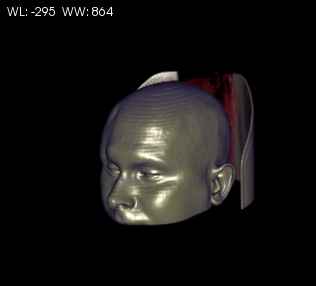
\includegraphics[width=0.332\textwidth]{raycasting_add_3}}
  \caption{Tissue Addition}
  \label{fig:raycasting_add}
\end{figure}

\newpage


\section{Cut}

%Em visualização volumétrica, o corte é utilizado para visualizar uma região interna do volume.
%O InVesalius dispõe de uma ferramenta para corte com base em um plano de referência. Com
%um padrão de visualização selecionado, clique em \textbf{Ferramentas} e, em seguida, em
%\textbf{Plano para corte} (figura \ref{fig:activate_cut_plane}).
In volume rendering, the cut is used to view a region of the internal volume. InVesalius has a cut for tool for this based on a reference plane. With a selected display pattern, click Tools, and then click Plan to cut (figure~\ref{fig:activate_cut_plane}).

\begin{figure}[!htb]
\centering
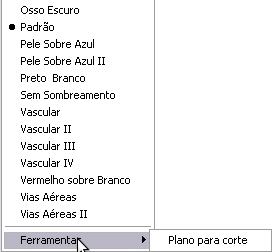
\includegraphics[scale=0.6]{activate_cut_plane_pt.png}
\caption{Enabling plan to cut}
\label{fig:activate_cut_plane}
\end{figure}

%Uma representação do plano para corte é exibida junto ao volume. Para realizar o corte,
%mantenha o botão \textbf{esquerdo} pressionado sobre o plano e \textbf{arraste} o mouse.
%Para rotacionar o plano, mantenha o botão \textbf{esquerdo} pressionado sobre a sua borda
%e movimente o mouse na direção desejada. Veja um exemplo na figura \ref{fig:cutted_image}.
A plan of representation for cutting appears next to the volume. To make the cut, hold the left mouse button on the plane and drag the mouse. To rotate the plan, hold the left mouse button  pressed on its edge and move the mouse in the desired direction. See an example in figure~\ref{fig:cutted_image}.

\begin{figure}[!htb]
\centering
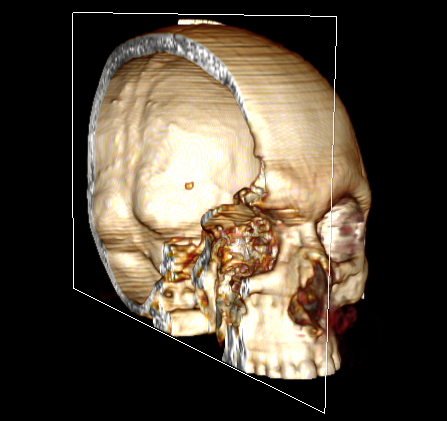
\includegraphics[scale=0.6]{cutted_image}
\caption{Image with clipping plane}
\label{fig:cutted_image}
\end{figure}

%Para desativar o recurso de corte, clique novamente em \textbf{Ferramentas} e em
%\textbf{Plano para corte} (figura \ref{fig:activate_cut_plane}).

To disable the cut feature, click Tools and then again Plan to cut (figure~\ref{fig:cutted_image}).